\chapter{L'algoritmo \emph{collapsed cone} e la sua implementazione in RayStation}
\setcounter{minitocdepth}{1}
\minitoc
\setcounter{minitocdepth}{2}
\textsf{In questo capitolo verrà descritto l'algoritmo di calcolo dosimetrico \textit{collapsed-cone-convolution} e la sua implementazione all'interno del treatment planning system (TPS) \RS. Ci si soffermerà in particolare sugli aspetti riguardanti le approssimazioni intrinseche dell'algoritmo assieme alle approssimazioni adottate in fase di implementazione nel TPS. Ciò è propedeutico alla comprensione dei limiti e delle precisioni raggiungibili durante la modellizzazione di un fascio clinico per trattamenti radioterapici che verrà discusso nei capitoli successivi.}

\section{Introduzione}
\label{sec:intro}
In radioterapia la \textit{dose assorbita} è quella quantità che viene utilizzata al pari della dose farmacologica per ottenere un determinato effetto terapeutico. Più precisamente, la definizione formale è fornita nel report ICRU n.85 \cite{ICRU85} come rapporto tra l'energia media $\de \bar{\varepsilon}$ impartita da radiazioni ionizzanti ad una massa $\de m$:
\begin{equation}
D = \frac{\de \bar{\varepsilon}}{\de m} \qquad\qquad \text{Unità: J\,kg}^{-1} \equiv \text{Gray [Gy]}
\end{equation} 
Esistono varie modalità di impartire una certa dose ad un paziente in radioterapia. Nell'ambito di questo lavoro si considererà solo la tecnica che fa impiego di fotoni generati da un acceleratore lineare (LINAC) denominata \virg{radioterapia a fasci esterni}.

Un LINAC è un'apparecchiatura in grado di accelerare elettroni fino ad energie dell'ordine dei 20 MeV che vanno a collidere su un target da cui si origina radiazione di frenamento (bremsstrahlung). Il fascio di fotoni così generato viene opportunamente filtrato e collimato per generare un fascio terapeutico. 
\begin{figure}
\centering
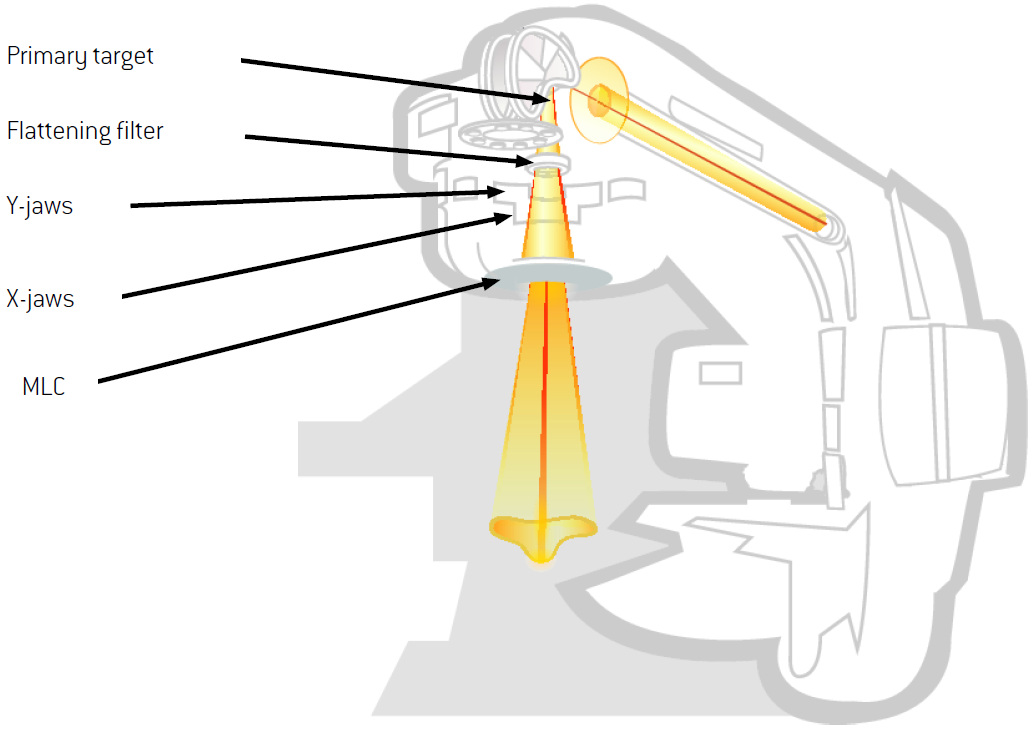
\includegraphics[width=.7\textwidth]{./cap1/linac.png}
\caption{Figura schematica di un acceleratore lineare per radioterapia a fasci esterni.}
\label{fig:linac}
\end{figure}
Tutto ciò si realizza nella testata del LINAC mediante l'uso di opportuni materiali schermanti che sono indicati nel disegno schematico riportato in Fig.\ref{fig:linac}.

Una volta che il fascio clinico investe il paziente, il meccanismo di deposizione della dose è un processo molto complesso dovuto alla grande quantità di fenomeni che vengono innescati in cascata. \`{E} importante notare che una parte non trascurabile di processi avviene anche a livello della testata e questi vanno ad influenzare il fascio che effettivamente giunge al paziente. Ad esempio uno degli effetti più clinicamente rilevanti è la generazione di elettroni che \textquotedblleft contaminano\textquotedblright{} il fascio fotonico.

\begin{figure}
\centering
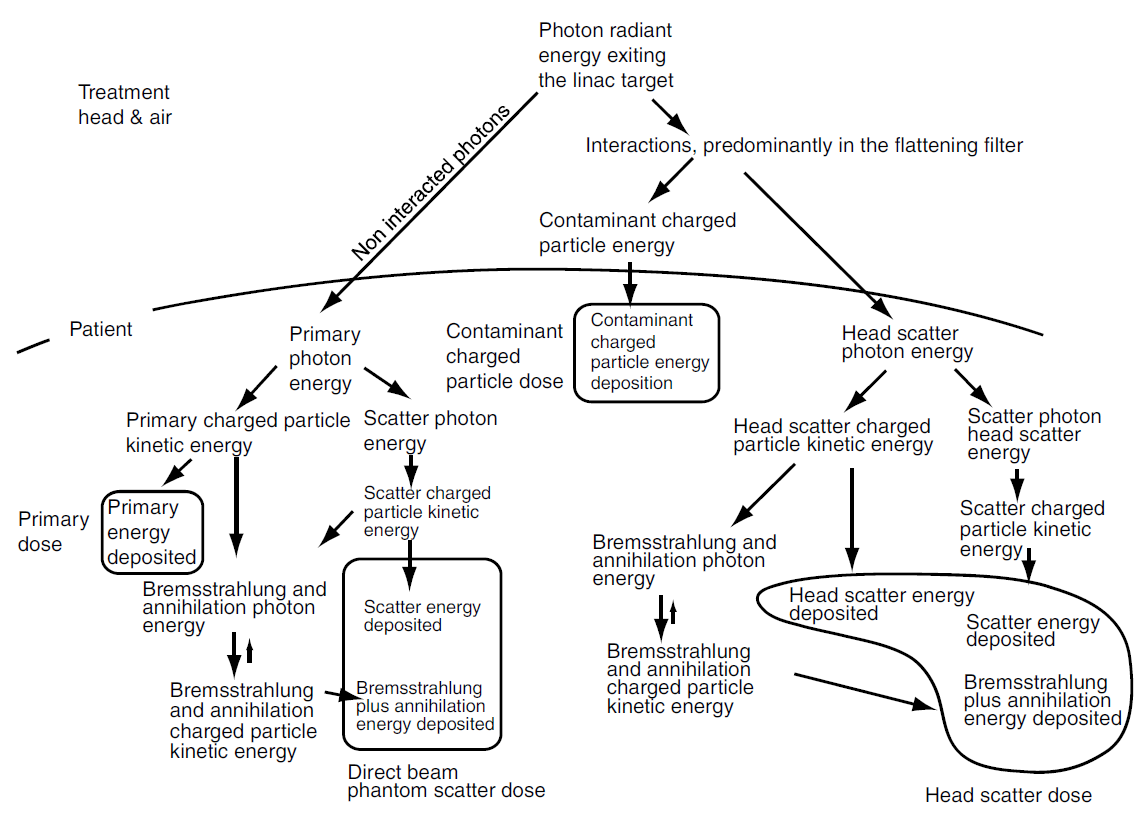
\includegraphics[width=.9\textwidth]{./cap1/processes.png}
\caption{Rappresentazione schematica delle principali interazioni che portano alla deposizione della dose nel paziente.}
\label{fig:processes}
\end{figure}
\vspace{.2cm}
La Fig.\ref{fig:processes} riassume schematicamente le principali interazioni che portano alla deposizione della dose nel paziente. \`{E} possibile identificare quattro principali meccanismi di rilascio della dose (cerchiati nella figura) che elenchiamo in ordine di importanza:
\begin{enumerate}
\item La dose primaria che rappresenta generalmente fino al 70\% della dose totale. Questa dose è generata dalla parte di fascio fotonico che non ha subito trasformazioni nella testata e che mette in moto particelle cariche le quali direttamente rilasciano la loro energia cinetica nella materia.
\item La dose di scatter dovuta al paziente (\textit{phantom scatter dose}) che può rappresentare fino al 30\% della dose totale. Questa componente è dovuta a tutti i processi di scatter che si innescano nel paziente a partire dal fascio primario come ad esempio fotoni di bremsstrahlung o fotoni scatterati per effetto Compton che portano ad una ionizzazione della materia con lo stesso meccanismo del fascio primario (messa in moto di elettroni).
\item La dose di scatter dovuta alla testata (\textit{head scatter dose}) che rappresenta generalmente il 5-10\% della dose totale. Questa parte della dose è dovuta alla componente di fascio fotonico che ha subito interazioni nella testata (prevalentemente nel \textit{flattening-filter}\footnote{\label{foot:flatt} Il \textit{flattening-filter} è un dispositivo di forma piramidale che serve ad attenuare il fascio al centro in modo da realizzare una fluenza di fotoni uniforme lungo la direzione perpendicolare al fascio.}) e presenta una distribuzione spaziale ed energetica differente dal fascio primario. Il meccanismo di rilascio dell'energia è analogo a quello del fascio primario.
\item La dose dovuta alle particelle di contaminazione del fascio fotonico che hanno un effetto rilevante (comparabile con il fascio primario) soltanto nei primi centimetri di tessuto. Questa zona è conosciuta come \textit{regione di build-up} della dose e vedremo in seguito il perché.
\end{enumerate}


\section{Generalità sugli algoritmi di calcolo della dose al paziente per fasci di fotoni}
Un algoritmo di calcolo dosimetrico ha lo scopo di predire, con un certo livello di accuratezza, gli effetti di interazione radiazione-materia presentati nella sezione precedente. In particolare, il fine ultimo è predire la distribuzione di dose totale assorbita nel paziente che costituisce l'entità correlata all'effetto terapeutico sul tumore o al danno sul tessuto sano. La possibilità di prevedere questa quantità è propedeutica al processo noto come \textit{pianificazione del trattamento} in cui vengono adoperate delle opportune scelte riguardanti la collimazione e l'intensità del fascio volte a minimizzare il rapporto rischio/beneficio della terapia.

Esistono due grandi classi di algoritmi dosimetrici:
\begin{itemize}
\item Algoritmi \textit{correction-based}.
\item Algoritmi \textit{model-based}.
\end{itemize}
Gli algoritmi correction-based sono algoritmi empirici. Essi sono  basati su un gruppo di dati misurati in certe condizioni di riferimento e fanno uso di fattori o funzioni matematiche di tipo analitico o di tipo look-up-table per predire la distribuzione di dose assorbita in altre condizioni. 
Questi metodi furono i primi ad essere implementati in quanto non necessitano di grosse potenze di calcolo ma, d'altro canto, presentano dei limiti di accuratezza intrinseci per situazioni complesse (mezzi non omogenei, interfacce tra tessuti, campi di irradiazione molto irregolari o ad intensità modulata\ldots). Un'estensiva review di questi tipi di algoritmi è stata pubblicata da Fraass \textit{et al.}\cite{Fraass1995}.

\vspace{.2cm}
L'avvento della rivoluzione tecnologica e la crescita della potenza di calcolo disponibile tramite computer, ha permesso l'implementazione degli algoritmi model-based i quali simulano i processi di interazione radiazione-materia  a partire da principi primi tramite un modello fisico-matematico.\\
In questo caso il set di misure iniziali è unicamente utilizzato per ottimizzare i parametri del modello che poi viene applicato per predire la distribuzione di dose assorbita nei vari scenari clinici. Questi algoritmi hanno dimostrato una maggiore accuratezza rispetto ai correction-based ed al giorno d'oggi i più utilizzati sono quelli basati su metodi semi-analitici (algoritmi di convolution/superposition) oppure algoritmi statistici basati su tecniche Monte Carlo.

Il TPS RayStation in particolare implementa una tecnica di tipo convolution/superposition conosciuta come \textit{collapsed cone convolution} sviluppata a partire dalla metà dagli anni '80 indipendentemente da Mackie e Ahnesj{\"{o} \cite{Ahnesjo1989, Boyer1998, Mackie1985, Ahnesjo1987}.

\subsection{I principi di \textit{convolution} e \textit{superposition}}
I principi di sovrapposizione e di convoluzione sono concetti matematici largamente utilizzati in fisica. In termini matematici, l'operazione di sovrapposizione consiste nella somma di una serie di funzioni, ognuna con un proprio peso.\\
Nel caso continuo, il principio di sovrapposizione può essere espresso con un integrale di volume tra una funzione primaria $p$ ed una funzione kernel $s$:
\begin{equation}
D(x,y,z) = \int_V p(x',y',z')\, s(x,x',y,y',z,z')\de x' \de y' \de z'
\end{equation}
Un particolare caso del principio di sovrapposizione è rappresentato dalla convoluzione che si realizza quando la funzione kernel è spazialmente invariante, ovvero dipende solo dalla differenza tra la coordinata $(x,y,z)$ e la variabile di integrazione $(x',y',z')$:
\begin{equation}
D(x,y,z) = \int_V p(x',y',z')\, s(x-x',y-y',z-z')\de x' \de y' \de z'
\end{equation}



\section{Teoria degli algoritmi \textit{convolution}/\textit{superposition}}
\label{sec:teoria_conv}

Il problema del calcolo della dose in un punto all'interno di un volume è in generale un problema di sovrapposizione.
\begin{figure}
\centering
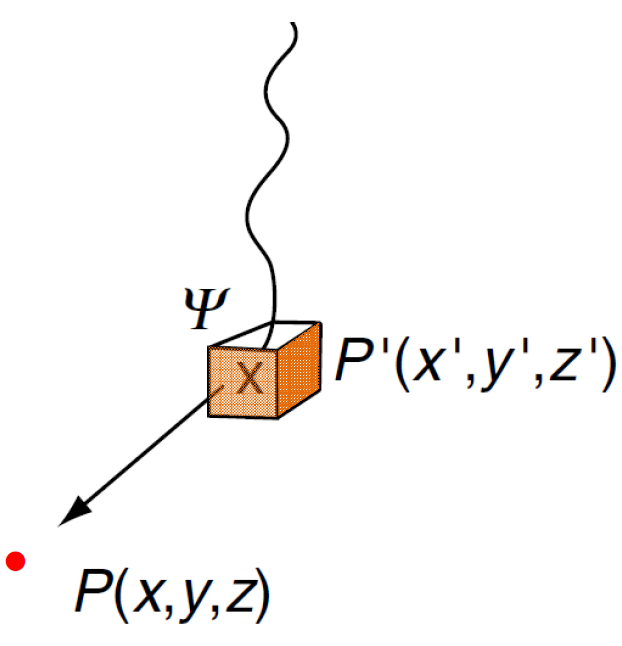
\includegraphics[width=.45\textwidth]{./cap1/superp1.png}
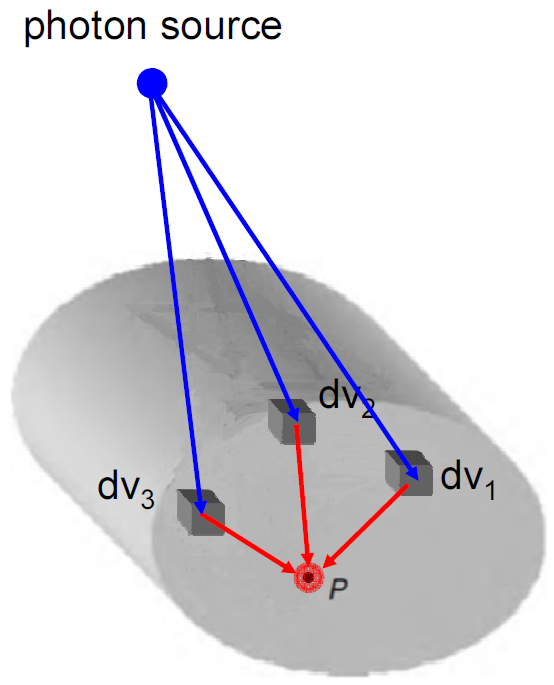
\includegraphics[width=.45\textwidth]{./cap1/superp2.png}
\caption{Il calcolo della dose visto come principio di sovrapposizione.}
\label{fig:superp}
\end{figure}
In particolare, osservando la Fig.\ref{fig:superp}, si nota come la quantità di energia che viene rilasciata in un punto $P$ dipenda da infiniti contributi dovuti alle particelle ionizzanti messe in moto dai fotoni nei loro rispettivi centri di interazione $P'\,(\de V_i)$.\\
L'insieme di interazioni dei fotoni primari nei punti $P'$ va a formare una quantità denominata TERMA (total-energy-released-in-matter) che rappresenta l'energia totale immagazzinata in un volume. Questa quantità viene trasformata in energia cinetica di particelle cariche (elettroni) e fotoni secondari (detti fotoni di scatter).\\
Il TERMA è esprimibile come il prodotto tra la \textit{fluenza di energia primaria} (quantità di energia radiante incidente per unità di superficie [J m$^{-2}$]) e il coefficiente di assorbimento lineare massico del mezzo $(\mu/\rho)$ \cite{Ahnesjo1987}.

Dalla conoscenza del TERMA ($T(x,y,z)$) e della funzione di scatter $s(x'\rightarrow x, y'\rightarrow y, z'\rightarrow z)$ che esprime l'ammontare di energia depositata nel punto $P(x,y,z)$ dovuta all'interazione avvenuta nel punto $P'(x',y',z')$, la dose assorbita nel punto $P$ è esprimibile con il principio di sovrapposizione:
\begin{align}
D(x,y,z) &=  \int_V \frac{\mu(x',y',z')}{\rho(x',y',z')} \Psi(x',y',z')\,s(x'\rightarrow x, y'\rightarrow y, z'\rightarrow z)\, \de x' \de y' \de z'\\
         &= \int_V T(x',y',z')\,s(x'\rightarrow x, y'\rightarrow y, z'\rightarrow z)\, \de x' \de y' \de z'\\
         &= \int_V T(P')\,s(P'\rightarrow P)\, \de V
\end{align}

Questa equazione è valida nel caso di un fascio di fotoni monoenergetico, tuttavia la generalizzazione è semplice introducendo il TERMA differenziale in energia $T(P',E)$ e la funzione di scatter polienergetica $s(P'\rightarrow P,E)$ ed integrando su tutte le energie coinvolte:
\begin{equation}
\boxed{D(P) = \iint_{E,V} T(P',E)\,s(P'\rightarrow P,E)\, \de V \de E}
\label{eq:superp}
\end{equation}
L'equazione \eqref{eq:superp} rappresenta il principio di sovrapposizione (\textit{superposition}) applicato al calcolo della dose in un volume investito da un fascio di fotoni polienergetico.

Un caso di particolare interesse è quello di un fascio di fotoni monoenergetico e parallelo che investe un mezzo omogeneo. In queste condizioni la funzione di scatter (conosciuta anche come \textit{energy deposition point kernel} o \textit{point spread kernel} o \textit{kernel di deposizione}) è spazialmente invariante per cui l'integrale di sovrapposizione diventa a tutti gli effetti un integrale di convoluzione, facilmente risolvibile grazie alla teoria degli spazi di Fourier.\\
Storicamente il passaggio è stato proprio partire da questo caso più semplice per poi aggiungere variabili come la divergenza del fascio, la caratteristica polienergetica e le disomogeneità del mezzo che ci riportano al problema più complesso (ma più accurato) della sovrapposizione. Per questo motivo gli algoritmi basati su questa teoria sono conosciuti come algoritmi di \textit{convolution/superposition}.



\section{Il calcolo della dose in RayStation}
\label{sec:algo_Ray}
Il calcolo della dose nel TPS RayStation fa uso del formalismo illustrato nelle sezioni precedenti e procede in quattro principali passaggi:
\begin{enumerate}
\item Il calcolo della fluenza di energia.
\item Il calcolo del TERMA.
\item L'applicazione delle opportune funzioni di scatter e del principio di sovrapposizione per il calcolo della dose finale.
\item La somma del contributo dovuto alle particelle di contaminazione (elettroni).
\end{enumerate}

\subsection{Il calcolo della fluenza di energia}
\label{sec:fluence}
Questo primo step consiste in un calcolo geometrico che non tiene conto della presenza del paziente. Si è già notato nella sezione introduttiva (Fig.\ref{fig:processes}) come il fascio in ingresso in un paziente sia costituito da una parte primaria e da una parte che ha interagito con gli elementi della testata (in particolare con il flattening-filter). RayStation tratta queste due componenti con un modello a due sorgenti poste ad una certa distanza lungo la direzione di propagazione del fascio (Fig.\ref{fig:twosources}).
\begin{figure}
\centering
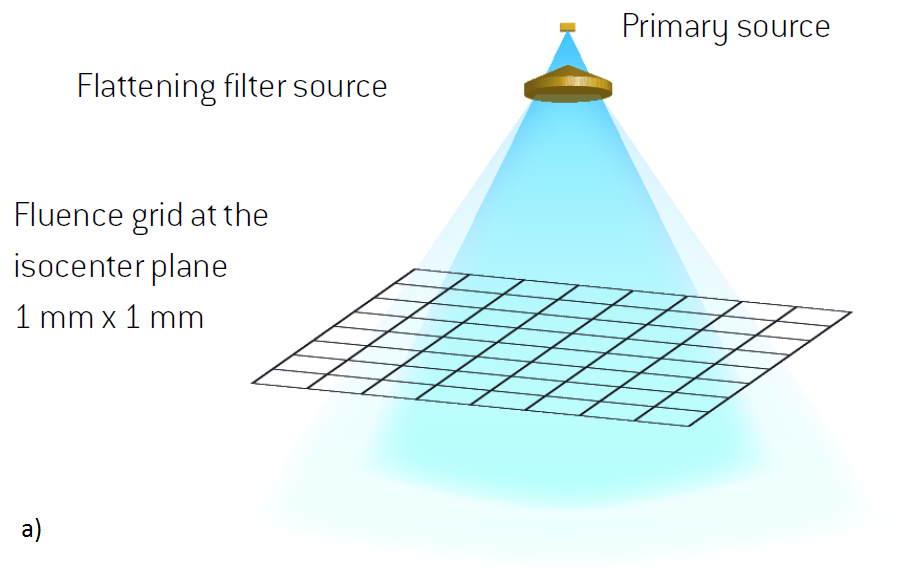
\includegraphics[width=.55\textwidth]{./cap1/twosources.png}
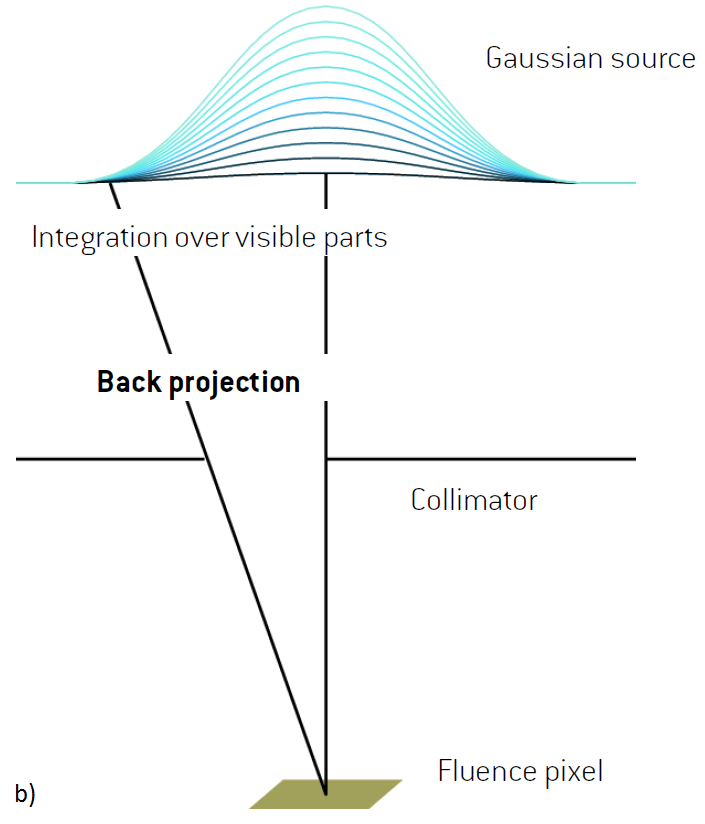
\includegraphics[width=.4\textwidth]{./cap1/source_int.png}
\caption{ (a) Modello a due sorgenti utilizzato per il calcolo della fluenza di energia. (b) Processo di integrazione della parte visibile della sorgente per il calcolo della fluenza.}
\label{fig:twosources}
\end{figure}
La sorgente primaria è modellizzata con un profilo gaussiano ellittico esteso dell'ordine dei mm mentre la sorgente di scatter del flattening-filter è gaussiana circolare estesa dell'ordine dei cm \cite{Chaney1994}.\\
Il calcolo della fluenza viene effettuato su un piano passante per il centro di simmetria rotazionale del LINAC denominato \textit{isocentro} e perpendicolare alla direzione del fascio (Fig.\ref{fig:twosources}a).
Le sorgenti vengono geometricamente proiettate attraverso i collimatori indicati in Fig.\ref{fig:linac} costituiti da blocchi di materiale schermante (\textit{jaws}) e da un dispositivo fatto di lamelle retraibili (\textit{multi-leaf-collimator}) che serve a generare conformazioni irregolari del fascio.\\
Matematicamente, l'operazione di calcolo della fluenza consiste in un'integrazione pixel per pixel della parte di sorgente \textquotedblleft visibile\textquotedblright{} attraverso i collimatori (Fig.\ref{fig:twosources}b) con un metodo di backprojection.\\
La mappa di fluenza così ottenuta viene corretta per includere alcuni fenomeni come la trasmissione dei collimatori, la trasmissione della punta e del bordo delle lamelle (\textit{leaf tip e tongue}\&\textit{groove}), il peso relativo delle sorgenti ed altri processi che verrano discussi in seguito.

In parallelo viene computata la mappa di fluenza per le sorgenti di elettroni di contaminazione. Queste ultime sono gaussiane circolari e poste alla stessa posizione delle sorgenti di fotoni. Esse sono divise in primaria e di scatter del flattening filter e la loro intensità è espressa in percentuale rispetto alla fluenza dei fotoni primari.

\subsection{Il calcolo del TERMA}
Il TERMA costituisce la prima parte dell'integrale per il calcolo della dose assorbita (Eq.\ref{eq:superp}). Esso quantifica in pratica l'assorbimento della fluenza di energia che attraversa il paziente. A partire da questo assorbimento vengono applicate le funzioni di scatter per generare la distribuzione di dose.\\
Il TERMA differenziale in energia è stato definito nella Sez.\ref{sec:teoria_conv} in accordo con \cite{Ahnesjo1999}:
\begin{equation}
\label{eq:termaE}
T(\vec{r'},E) = \frac{\mu}{\rho}(\vec{r'},E)\,\Psi(\vec{r'},E)
\end{equation}
dove $\vec{r'}$ è la coordinata del punto di interazione primaria.

Il paziente è modellizzato all'interno del TPS tramite uno studio di tomografia computerizzata che contiene una mappa di densità dei tessuti. Questo permette di conoscere il primo termine dell'Eq.\eqref{eq:termaE} \cite{RaySearchLaboratories2014}.\\
Il secondo termine è la fluenza di energia calcolata nello step precedente. Per il calcolo del TERMA, detta fluenza viene proiettata verso la sorgente primaria fino a coincidere con la superficie del paziente ($\Psi(\vec{r_0},E)$) e poi viene riproiettata verso il basso tenendo conto dell'assorbimento nei tessuti (esponenziale con il coefficiente di assorbimento) e della divergenza del fascio (decadimento col quadrato della distanza):
\begin{equation}
\label{eq:fluence}
\Psi(\vec{r'},E) = \frac{|\vec{r_0}|^2}{|\vec{r'}|^2}\Psi(\vec{r_0},E)\,\exp{\left( -\int_{\vec{r_0}}^{\vec{r'}} \mu(\vec{r'},E) \de l \right)}
\end{equation}
L'integrale del coefficiente di assorbimento nella precedente equazione viene discretizzato nel TPS su una griglia di voxel cubici detta \textit{dose grid}. Questi voxel campionano le densità fornite dalla CT da cui viene ricavato il coefficiente di assorbimento locale (vedi Fig.\ref{fig:terma}). A questo punto, moltiplicando entrambi i termini dell'equazione \eqref{eq:termaE} si ottiene la distribuzione di TERMA.

\begin{figure}
\centering
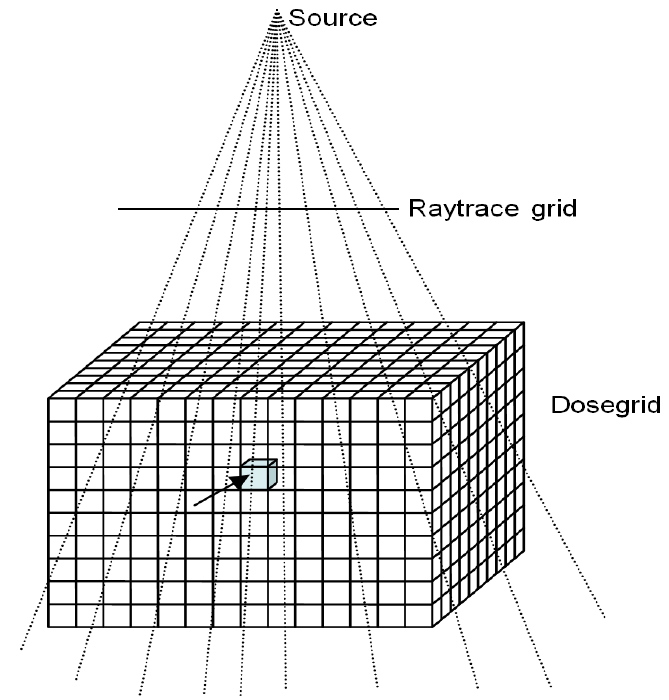
\includegraphics[width=.4\textwidth]{./cap1/terma_1.png}
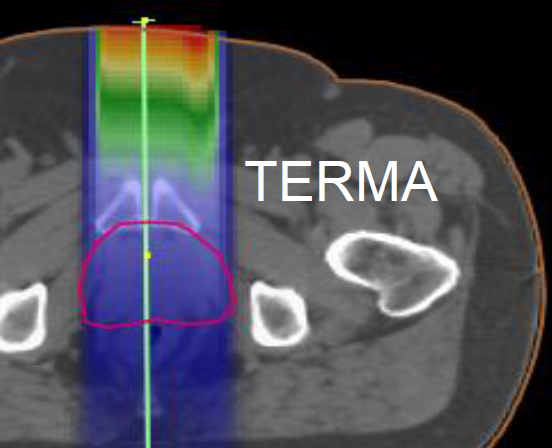
\includegraphics[width=.5\textwidth]{./cap1/terma_2.png}
\caption{Sinistra: griglia per il calcolo del TERMA e della dose. Da notare che, per motivi di velocità, la divergenza del fascio viene approssimata come proveniente unicamente dalla sorgente primaria e non dal flattening filter. Destra: distribuzione del TERMA computato su una scansione CT di un paziente.}
\label{fig:terma}
\end{figure}

\subsection{Applicazione delle funzioni di scatter}
Se l'energia totale rilasciata dai fotoni in un voxel fosse interamente assorbita in esso, la distribuzione di TERMA coinciderebbe con la dose assorbita.\\
\begin{figure}
\centering
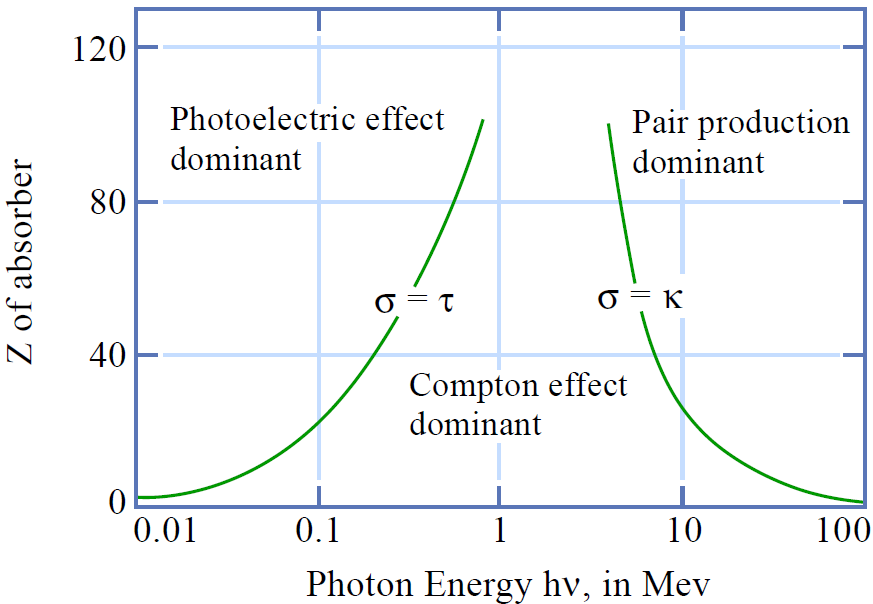
\includegraphics[width=.7\textwidth]{./cap1/compt_dom.png}
\caption{Prevalenza degli effetti di interazione dei fotoni con la materia in funzione dell'energia del fotone. L'effetto Compton è prevalente per le energie e i materiali tipici della radioterapia.}
\label{fig:compt_dom}
\end{figure}
Tuttavia alle energie tipiche dei fotoni utilizzati in radioterapia l'effetto predominante è l'effetto Compton (Fig.\ref{fig:compt_dom}).

Una modellizzazione completa del trasporto del fotone diffuso e dell'elettrone messo in moto richiede un approccio statistico di tipo Monte Carlo, computazionalmente molto dispendioso.\\
L'approccio convolution/superposition racchiude i processi statistici di deposizione dell'energia nella funzione di scatter introdotta nell'Eq.\eqref{eq:superp} ed agisce in maniera deterministica.\\
Questa funzione è ottenibile a partire da una simulazione Monte Carlo in cui un unico fotone viene fatto interagire forzatamente all'interno di un volume omogeneo di acqua e si va a registrare la deposizione della dose che ne deriva.\\
Questa operazione è stata effettuata da Mackie \cite{Mackie1985} utilizzando il software Monte Carlo EGS sviluppato dallo Stanford Linear Accelerator Center che pubblicò nella metà degli anni '80 delle funzioni di scatter discretizzate in forma tabulare, proponendo un metodo di convoluzione del tipo look-up-table (prontamente implementabile in un computer). Propose anche un metodo per riscalare le funzioni di scatter con la densità per poter calcolare la dose in mezzi diversi dall'acqua senza dover rieffettuare la simulazione Monte Carlo (vedi Fig.\ref{fig:mackie_kernels}).
\begin{figure}
\centering
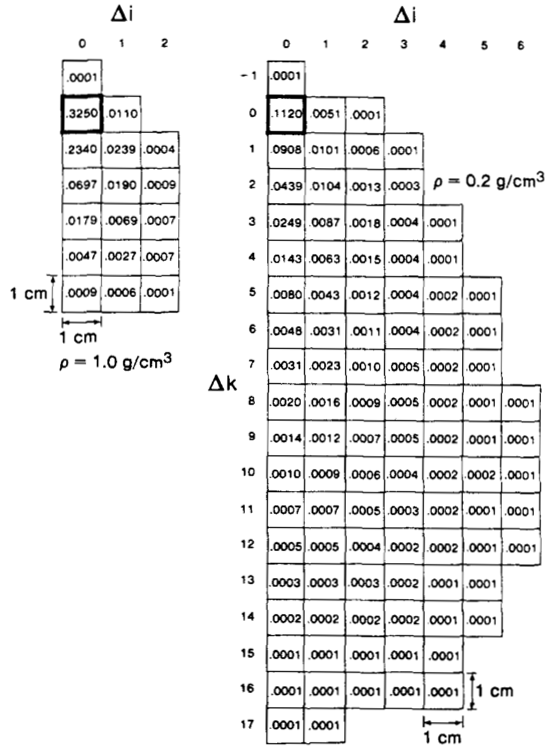
\includegraphics[width=.8\textwidth]{./cap1/mackie_kernels.png}
\caption{Funzione di scatter calcolate da Mackie \cite{Mackie1985} per un fotone da 15MV. Da notare come l'assunzione di deposizione locale dell'energia non è accettabile (nel punto di interazione cade il 32.5\% della dose totale per l'acqua e l'11.2\% per un mezzo di densità 0.2g/cc.)}
\label{fig:mackie_kernels}
\end{figure}

Applicando le funzioni di scatter (kernel) ai punti di deposizione del TERMA, è possibile arrivare alla dose assorbita in maniera triviale utilizzando il metodo di sovrapposizione. Tuttavia, questa operazione su una griglia di $N^3$ voxel risulta essere un problema  di ordine $N^6$ \cite{Ahnesjo1999}. Se si aggiunge l'operazione di scaling dei kernel per la densità il problema diventa di ordine $N^7$ difficilmente gestibile anche con le moderne potenze di calcolo\footnote{Se immaginiamo di discretizzare un paziente di dimensioni $20x20x20$ cm$^3$ con voxel di lato $0.3$ cm otteniamo una griglia di circa $70x70x70$ voxel. Il numero di operazioni da effettuare con un metodo di sovrapposizione triviale sarebbe $70^7\approx 10^{13}$. Disponendo di un computer capace di effettuare operazioni con frequenza dell'ordine del GHz$\equiv 10^9$ il tempo di risolvere $10^{13}$ operazioni sarebbe $t=10^{13}/10^9=10^5\,sec\approx 2\, ore!$.}. Per questo motivo, gran parte della ricerca successiva allo sviluppo del metodo di convolution/superposition fu orientata a sviluppare delle approssimazioni che permettessero il calcolo della dose in tempi compatibili con una routine di tipo clinico.

\subsection{L'approssimazione \textit{collapsed-cone}}
Lo stesso Mackie assieme a Reckwerdt \cite{Reckwerdt1992} propose un'approssimazione che consisteva nel calcolare l'integrale di sovrapposizione solo lungo determinate direzioni. Indipendentemente, Ahnesj\"{o} nel 1989 seguendo lo stesso approccio, pubblicò un articolo \cite{Ahnesjo1989} in cui propose un metodo di soluzione del problema convolution/superposition denominato \textit{collapsed-cone} e lo confrontò con la tecnica Monte Carlo ottenendo risultati eccellenti per l'epoca. Questi risultati rappresentano ancora oggi il benchmark per il calcolo della dose con TPS utilizzando metodi non statistici.
\begin{figure}[!t]
\centering
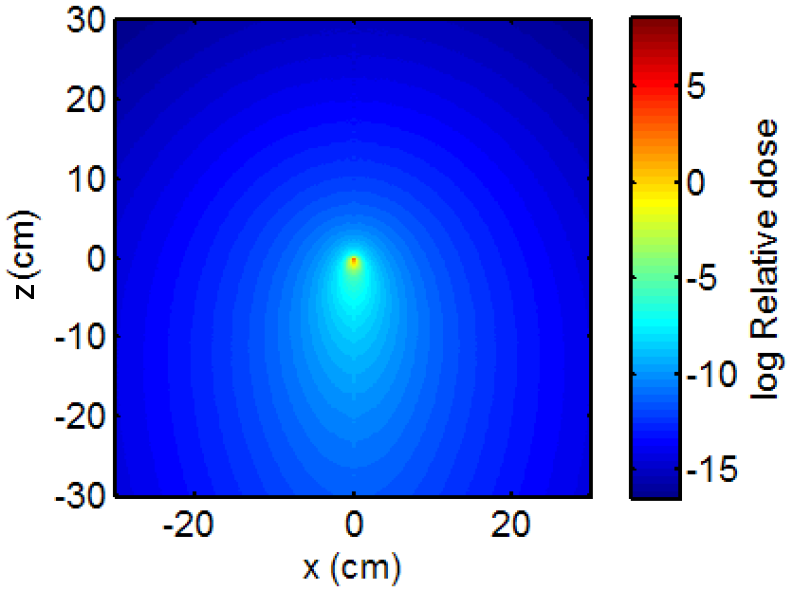
\includegraphics[width=.45\textwidth]{./cap1/kern_ray1.png}$\quad$
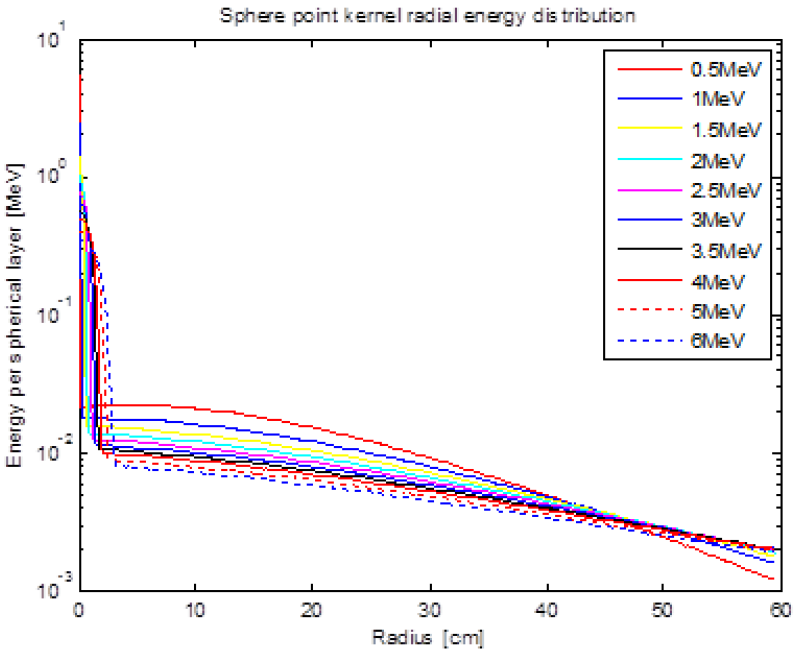
\includegraphics[width=.45\textwidth]{./cap1/kern_ray2.png}
\caption{Sinistra: distribuzione planare di un kernel di deposizione. Destra: distribuzione 1D di alcuni kernel al variare dell'energia; da notare una prima parte di rilascio rapido di energia dovuta agli elettroni Compton ed una parte più estesa dovuta ai fotoni secondari diffusi che a loro volta re-interagiscono con il mezzo.}
\label{fig:kern_ray}
\end{figure}
In Fig.\ref{fig:kern_ray} è possibile osservare la distribuzione spaziale tipica di alcuni kernel di deposizione.

L'approssimazione di collapsed cone consiste in una discretizzazione del kernel che è necessaria per poter risolvere l'equazione di sovrapposizione \eqref{eq:superp} per via computazionale. Ahnesj\"{o} notò che un metodo triviale di discretizzazione con dei semplici raggi, può portare ad un errore di sampling ampio a causa della rapidità di rilascio di energia nei primi cm di interazione \cite{Ahnesjo1989} (Fig.\ref{fig:kern_ray}) (i.e. una larga parte di deposizione di energia non viene conteggiata a meno di usare un campionamento angolare fittissimo).\\
Per questo Ahnesj\"{o} propose di discretizzare i kernel in coordinate sferiche con dei coni aventi il vertice nel punto di interazione e sottendenti un certo angolo solido. Tutte le deposizioni di energia contenute all'interno della superficie conica che sottende l'angolo solido vengono \textquotedblleft\textit{collassate}\textquotedblright{} sull'asse del cono stesso. Con questa procedura, l'energia totale depositata risulta spazialmente ridistribuita ma viene conteggiata per intero.

Matematicamente l'approssimazione di collapsed cone proposta da Ahnesj\"{o} consiste dapprima in un fit analitico del kernel di deposizione che in coordinate sferiche ha la seguente forma:
\begin{equation}
\label{eq:kern_fit}
s(r,\theta) = \frac{A_\theta e^{-a_\theta r} + B_\theta e^{-b_\theta r}}{r^2}
\end{equation}
dove $A_\theta,\,a_\theta,\,B_\theta$ e $b_\theta$ sono parametri di fit che dipendono dall'angolo di scatter $\theta$. I due termini esponenziali descrivono l'uno la caduta rapida del kernel dovuto agli elettroni Compton primari e l'altro la coda più lenta dovuta alle interazioni di scatter secondarie (Fig.\ref{fig:kern_ray}). Da notare che il kernel possiede una simmetria cilindrica per cui l'angolo $\phi$ non è esplicitato. La validità di questo fit è mostrata in Fig.\ref{fig:kern_fit}.
\begin{figure}
\centering
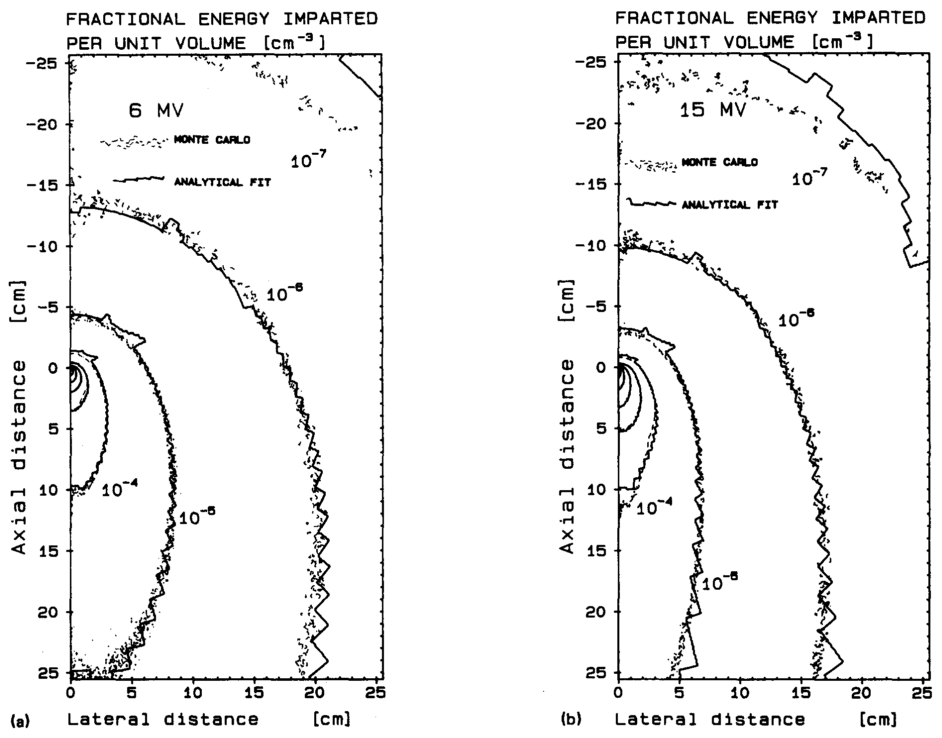
\includegraphics[width=.8\textwidth]{./cap1/kern_fit.png}
\caption{Fit analitico dei kernel di deposizione per un fotone da 6MV (a) e da 15MV (b). Tratto da \cite{Ahnesjo1989}.}
\label{fig:kern_fit}
\end{figure}

Stabilendo un angolo solido $\Omega_i$, l'operazione di \virg{collapsing} è un'integrazione in coordinate sferiche del kernel espresso dalla \eqref{eq:kern_fit} (vedi anche Fig.\ref{fig:kern_collaps}):
\begin{equation}
\iint_{\Omega_i} s(r,\theta) r^2\de \Omega_i = A_{\Omega_i} e^{-a_{\Omega_i} r} + B_{\Omega_i} e^{-b_{\Omega_i} r} \equiv K(r,\Omega_i)
\end{equation}
La funzione $K(r,\Omega_i)$ è quella da convolvere con la mappa del TERMA per arrivare alla mappa di dose assorbita.

Il metodo collapsed-cone è stato dimostrato \cite{Ahnesjo1999} comportare un numero di operazioni dell'ordine di $MN^3$ dove $M$ è il numero di settori in cui viene diviso l'angolo solido ed $N$ è il numero di voxel della griglia di dose/TERMA. Questo è da confrontare con l'ordine $N^7$ in caso di applicazione triviale del metodo di sovrapposizione.

\begin{figure}
\centering
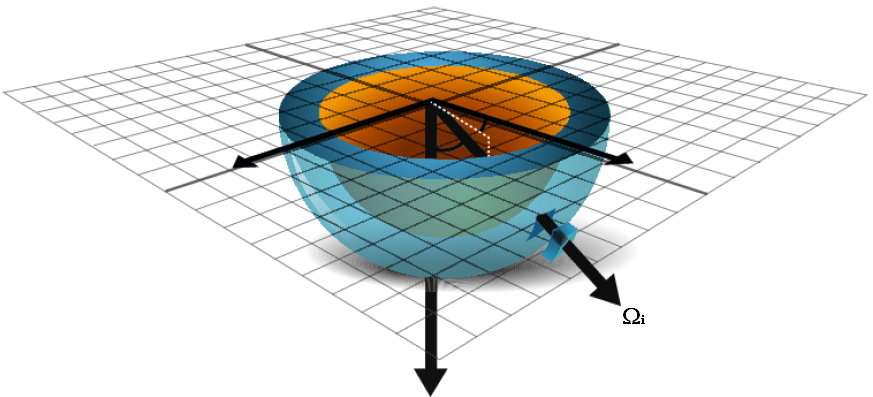
\includegraphics[width=\textwidth]{./cap1/kern_collaps.png}
\caption{Operazione di \textit{collapsing} dei kernel all'interno di segmenti conici definiti dall'angolo solido $\Omega_i$.}
\label{fig:kern_collaps}
\end{figure}

In RayStation il numero di settori in cui viene discretizzato il kernel è 128 che corrispondono a 8 direzioni lungo l'angolo di scatter $\theta$ e 16 lungo l'angolo di simmetria cilindrica $\phi$. Il campionamento è più fitto nella direzione di propagazione del fascio dove è presente il gradiente più intenso.

\subsection{La generalizzazione al caso polienergetico}
Un tipico fascio di fotoni generato da un LINAC per radioterapia contiene uno spettro polienergetico. Inoltre lo spettro subisce uno spostamento verso energie più alte a causa dell'attraversamento della materia (effetto di \textit{depth-hardening}). Questo suggerisce il fatto che non è possibile considerare un unico kernel di deposizione nel passaggio dal TERMA alla dose. Boyer et al. assieme a Zhu e Van Dyk \cite{Boyer1989,Zhu1995} hanno dimostrato che una discretizzazione in 5 bin sia sufficiente a rappresentare lo spettro di un LINAC da 6MV. Sulla base di ciò, Papanikolaou et al. \cite{Papanikolaou1993} hanno investigato i possibili metodi di estensione del metodo convolution al caso polienergetico dimostrando che è sufficiente combinare kernel monoergetici pesati con le relative componenti spettrali. Nel medesimo lavoro viene dimostrato che il problema del depth-hardening può essere risolto riscalando i kernel con dei fattori che dipendono dalla lunghezza radiologica attraversata.

Per applicare questi principi, nel TPS sono memorizzati una serie di point spread kernel computati con il motore Monte Carlo EDKnrc incluso in EGS4nrc per le seguenti energie del fotone primario incidente: 0.5, 1, 1.5, 2, 2.5, 3, 3.5, 4, 5, 6, 7, 8, 9 10, 12, 14, 16, 18, 20 MeV. Queste energie corrispondono ai bin implementati in RayStation per rappresentare uno spettro fotonico (es. per un fascio da 6 MV i bin coinvolti vanno da 0.5 a 6 MV).\\
Il peso di ogni componente spettrale viene stabilito in fase di modellizzazione (vedi cap. successivi). Per ora ci interessa sapere che, fissato lo spettro, viene costruito il kernel polienergetico secondo le indicazioni di Papanikolaou et al. \cite{Papanikolaou1993} (media pesata con le componenti spettrali). In seguito viene costruita una libreria di 600 kernel in un intervallo di lunghezze radiologiche da -100 g/cm$^2$ a 200 g/cm$^2$\footnote{Nota: lunghezze radiologiche negative sono necessarie per tenere in conto l'effetto di \textit{off-axis softening} dovuto alla presenza del flattening-filter di cui si parlerà nei capitoli successivi.} da essere utilizzati nel calcolo della dose.


\subsection{La generalizzazione al caso disomogeneo}
Un ulteriore fenomeno da tenere in conto nell'applicazione dei point spread kernel è la disomogeneità del mezzo. In condizioni standard i kernel sono calcolati in un volume omogeneo di acqua, tuttavia la deposizione di energia cambia se i processi di ionizzazione avvengono in un mezzo differente dall'acqua.\\
Woo e Cunningham \cite{Woo1990} assieme a Mackie \cite{Mackie1985} hanno dimostrato come sia possibile evitare di ricalcolare i kernel per ogni situazione sostituendo tutte le lunghezze fisiche ($l$) con le lunghezze radiologiche ($\rho\,l$) (dove $\rho$ è la densità del mezzo). La base di questa metodologia era in realtà nota già prima dell'avvento degli algoritmi di convolution come Teorema di O'Connor \cite{OConnor1957}.\\
\begin{figure}[!t]
\centering
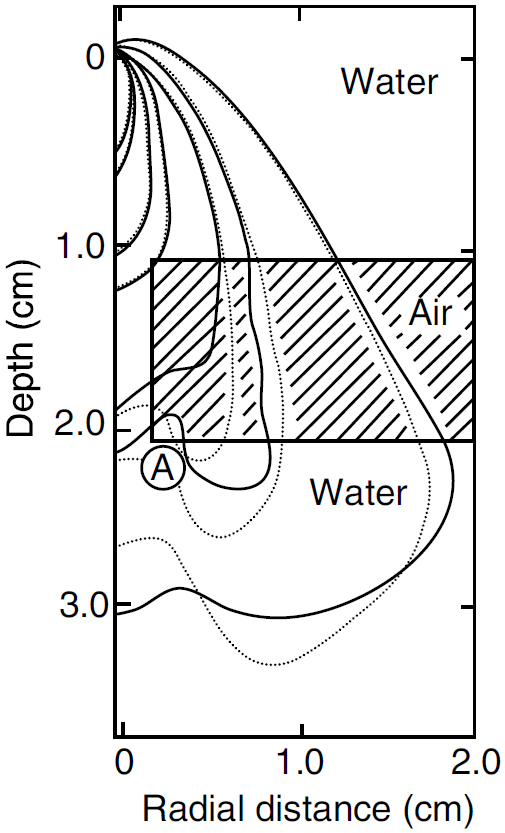
\includegraphics[width=.4\textwidth]{./cap1/kern_dens.png}
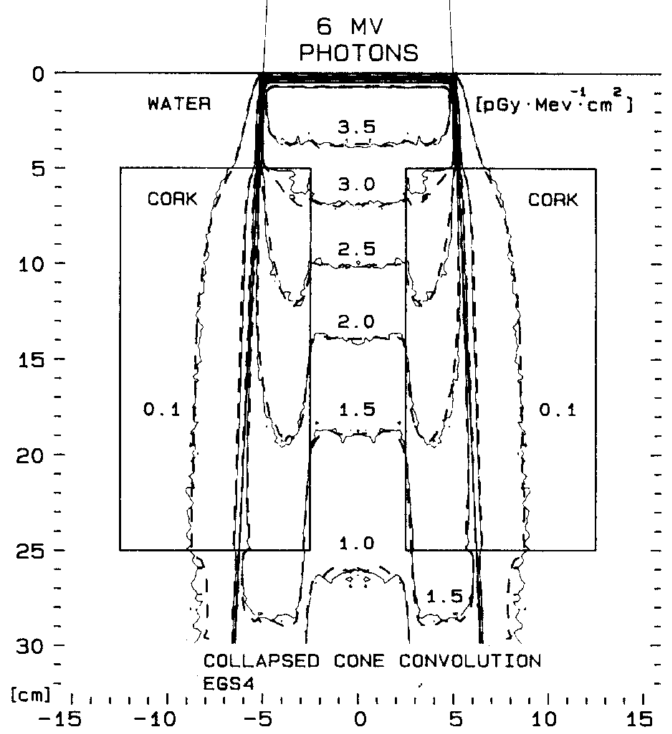
\includegraphics[width=.59\textwidth]{./cap1/kern_dens2.png}
\caption{Sinistra: Contronto tra un kernel calcolato direttamente con un metodo Monte Carlo (linea solida) e un kernel calcolato in condizioni omogenee riscalato secondo la lunghezza radiologica (linea tratteggiata); le isolinee corrispondono ad una dose relativa di 1000, 500, 100, 50, 10, 5, 1; il punto A posizionato appena sotto l'interfaccia aria/acqua presenta la massima discrepanza (50\%). Destra: effetto globale su un insieme di interazioni; un \textit{averaging} delle incertezze sui singoli kernel si risolve in un accordo accettabile su un fantoccio complesso che simula un torace \cite{Woo1990,Arnfield2000,Ahnesjo1989}.}
\label{fig:kern_dens}
\end{figure}
Nella Fig.\ref{fig:kern_dens} si può notare l'errore che si commette adottando il metodo suggerito in una configurazione di disomogeneità aria/acqua che può simulare una situazione tessuto/polmone. Nonostante l'accordo non sia perfetto, Woo e Cunnigham \cite{Woo1990} assieme ad Arnfield et al. \cite{Arnfield2000} e lo stesso Ahnesj\"{o} \cite{Ahnesjo1989} hanno dimostrato che su un insieme numeroso di interazioni interviene un effetto di \textit{averaging} per cui discrepanze significative rimangono solo in condizioni di estrema disomogeneità, ossia vicino alle interfacce in cui la densità cambia repentinamente (vedi Fig.\ref{fig:kern_dens}).

Aggiungendo  la generalizzazione al caso disomogeneo l'equazione di sovrapposizione \eqref{eq:superp} per il calcolo della dose può essere riscritta \cite{Khan2010}:
\begin{equation}
D(\vec{r}) = \iint_{E,V} T_E(\rho_{\vec{r'}} \cdot \vec{r})\, s_E(\rho_{\vec{r}-\vec{r'}}\cdot (\vec{r}-\vec{r'}))\de\vec{r'} \de E
\end{equation}
dove $(\rho_{\vec{r'}} \cdot \vec{r})$ è la lunghezza radiologica dalla sorgente fino al punto di interazione primaria (ove viene rilasciato il TERMA) e $\rho_{\vec{r}-\vec{r'}}\cdot (\vec{r}-\vec{r'})$ è la lunghezza radiologica dal punto di interazione primaria al punto di deposizione della dose.

\begin{figure}
\centering
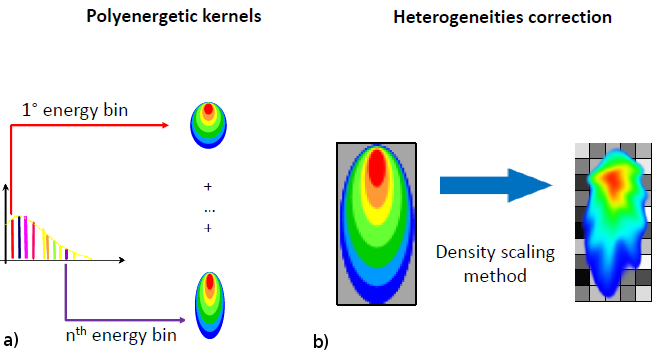
\includegraphics[width=\textwidth]{./cap1/kern_trans.png}
\caption{Sinistra: figura schematica del metodo con cui si costruisce il kernel polienergetico (combinazione di kernel monoenergetici pesati con la componente spettrale). Destra: figura schematica che rappresenta come il kernel si modifica quando viene riscalato tenendo conto delle lunghezze radiologiche attraversate nelle varie direzioni.}
\label{fig:kern_trans}
\end{figure}

In Fig.\ref{fig:kern_trans} sono riportati due diagrammi schematici riguardo le generalizzazioni al caso polienergetico e disomogeneo.


In Fig.\ref{fig:terma_dose} è riportato graficamente il processo di passaggio dal TERMA alla dose. Quello che si può notare è che l'applicazione dei kernel di deposizione comporta un \textquotedblleft\textit{blurring}\textquotedblright{} e un prolungamento della distribuzione di TERMA che è dovuto proprio al movimento delle particelle ionizzanti secondarie messe in moto dai fotoni primari e diffusi.
\begin{figure}
\centering
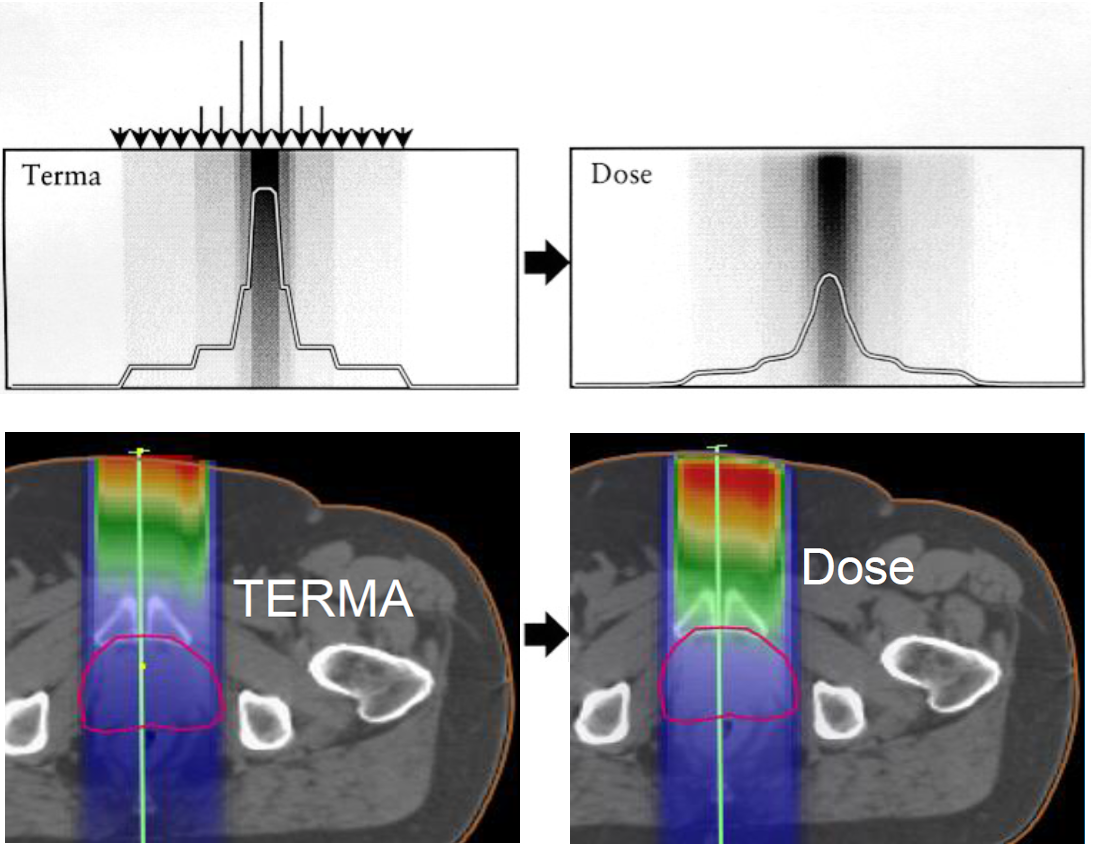
\includegraphics[width=.8\textwidth]{./cap1/terma_dose.png}
\caption{In alto: trasformazione del TERMA in dose in condizioni di omogeneità. In basso: trasformazione del TERMA in dose su una scansione CT di un paziente reale. Da notare è l'effetto di \textquotedblleft\textit{blurring}\textquotedblright{} dovuto all'applicazione dei kernel di deposizione.}
\label{fig:terma_dose}
\end{figure}



\section{Approssimazioni aggiuntive}
Nella sezione precedente sono state mostrate le approssimazioni intrinseche dell'algoritmo \textit{collapsed-cone}. In questa sezione evidenziamo delle ulteriori approssimazioni adottate in RayStation orientate all'aumento della velocità di calcolo della dose.

\subsection{L'approssimazione \textit{no-kernel-tilting}}
Un fascio di fotoni generato da un LINAC è tipicamente divergente all'aumentare della distanza dalla sorgente. I kernel di deposizione dell'energia sono calcolati per un fascio che incide verticalmente ed hanno l'asse orientato nella medesima direzione. Un'applicazione rigorosa del metodo convolution/superposition richiederebbe la rotazione dei kernel per allinearli lungo l'angolo di incidenza del raggio primario (vedi Fig.\ref{fig:kern_tilt}).\\
\begin{figure}
\centering
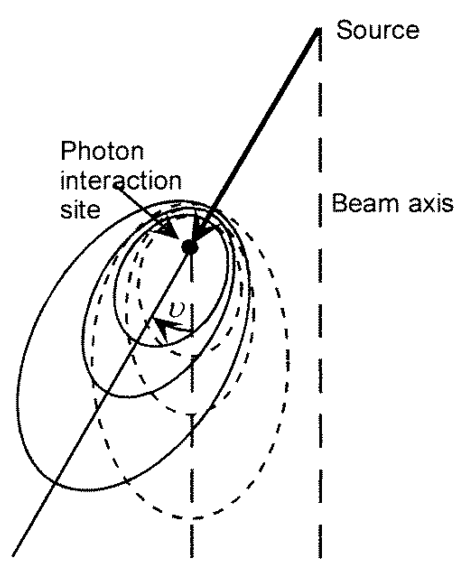
\includegraphics[width=.35\textwidth]{./cap1/kern_tilt.png}
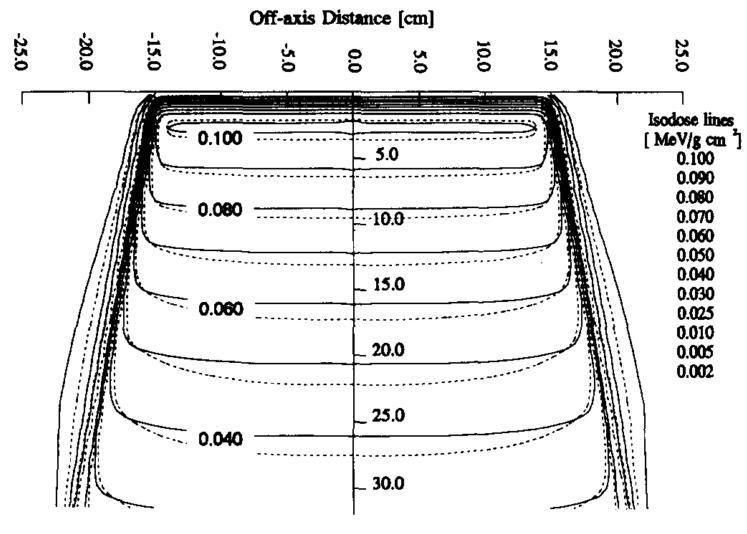
\includegraphics[width=.6\textwidth]{./cap1/kern_tilt_b.png}
\caption{Sinistra: I kernel di deposizione dovrebbero essere ruotati dello stesso angolo di incidenza $\nu$ del raggio primario; tuttavia per ridurre considerevolmente i tempi di calcolo, si applicano kernel con orientazione verticale. Destra: il non ruotare i kernel comporta una deposizione di dose maggiore verso il centro del fascio (linea tratteggiata) confrontata con la dose calcolata senza approssimazione (linea solida); questo può essere corretto secondo \cite{Papanikolaou1993} (vedi testo).} 
\label{fig:kern_tilt}
\end{figure}
Questa operazione implicherebbe molteplici rotazioni di matrici \cite{Sharpe1997} con il risultato di aumentare considerevolmente il tempo di calcolo della dose. 
%Oltre a questo, un ulteriore grande vantaggio dell'approssimazione \textit{no-kernel-tilting} consiste nel fatto di poter calcolare solo una volta le intersezioni dei raggi uscenti dai kernel con la griglia di dose\footnote{Operazione nota come \textit{raytracing}.} e di riutilizzare i risultati per i voxel successivi.
Per questo motivo vari autori hanno sviluppato dei metodi che consentissero di applicare kernel di deposizione non ruotati (\textit{no-kernel-tilting}) \cite{Sharpe1997,Papanikolaou1993}.

In RayStation è implementato il metodo suggerito da Papanikolaou et al. \cite{Papanikolaou1993}. L'idea di questo metodo sta nel considerare che, non ruotando i kernel, si ha un accumulo di dose maggiore verso il centro del fascio (Fig.\ref{fig:kern_tilt}).\\ 
Papanikolaou ha dimostrato come questo può essere recuperato con i seguenti passaggi:
\begin{enumerate}
\item Si rimuove la divergenza dalla fluenza di energia (termine $|\vec{r_0}|^2/|\vec{r'}|^2$ nell'Eq.\eqref{eq:fluence}).
\item Si applicano i point spread kernel con l'approssimazione di \textit{no-tilting}.
\item Si riapplica la divergenza riscalando la dose calcolata con il fattore $|\vec{r_0}|^2/|\vec{r}|^2$ dove $\vec{r}$ è la coordinata di calcolo della dose (diversa dalla coordinata di rilascio del TERMA $\vec{r'}$).
\end{enumerate}
L'effetto dell'operazione n.1 è quello di aumentare la fluenza di energia lontano dal centro del fascio. Applicando poi i punti 2 e 3 si arriva ad una distribuzione in cui la dose approssima quella calcolata considerando i kernel ruotati.\\
Sharpe e Papanikolaou \cite{Sharpe1997,Papanikolaou1993} hanno evidenziato come l'approssimazione di \textit{no-tilting} dei kernel presenti i suoi limiti solo in situazioni difficilmente realizzabili clinicamente. In particolare, discrepanze oltre il 3\% si osservano in caso di basse distanze sorgente-superficie del paziente (SSD $< 70$ cm) congiuntamente all'utilizzo di campi estesi ($> 20x20$ cm$^2$).



\subsection{Approssimazioni \textit{full-TERMA-deposition} e \textit{adaptive interpolation}}
Ulteriori approssimazioni denominate \textit{full-TERMA-deposition} e \textit{adaptive interpolation} sono volte ad evitare di applicare rigorosamente il metodo di collapsed-cone-superposition su ogni voxel della griglia di dose.\\
A questo proposito, la \textit{full-TERMA-deposition} può essere riassunta in quattro principali step:
\begin{enumerate}
\item Alla fine del calcolo della distribuzione di TERMA vengono identificati quei voxel in cui è stato depositato un TERMA minore dello 0.5\% del massimo TERMA rilasciato nel volume.
\item A partire da questi voxel viene costruita una iso-superficie che viene poi espansa di una lunghezza radiologica di 5 cm isotropicamente.
\item Al di fuori della superficie precedentemente calcolata non viene effettuato il trasporto del TERMA con l'algoritmo collapsed-cone bensì si assume un rilascio locale di tutta l'energia.
\item All'interno del volume compreso tra la superficie TERMA$_i= 0.5\%$ TERMA$_{max}$ e la sua espansione di $5$ cm  il trasporto avviene solo su alcune delle 128 direzioni del kernel di deposizione. 
\end{enumerate}
Questa approssimazione è stata osservata generare un'errore sul calcolo della dose minore dello 0.2\% su punti peraltro a bassa rilevanza clinica \cite{RaySearchLaboratories2014}.\\

\begin{figure}
\centering
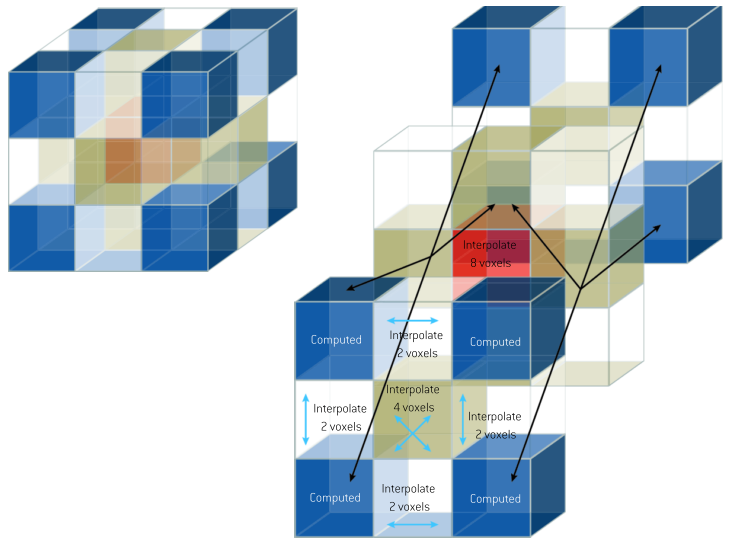
\includegraphics[width=\textwidth]{./cap1/dose_interp.png}
\caption{L'approssimazione di \textit{adaptive interpolation}. I voxel in blu sono quelli calcolati con l'algoritmo collapsed-cone.}
\label{fig:dose_interp}
\end{figure}

La seconda approssimazione di \textit{adaptive interpolation} si basa su un preliminare calcolo della dose su voxel alternati per identificare zone a basso od alto gradiente. Per le zone a basso gradiente la dose nei voxel non coinvolti nel computo preliminare viene calcolata con la media dei voxel adiacenti; per le zone ad alto gradiente viene applicato l'algoritmo completo. In particolare gli step che vengono seguiti sono riassumibili nei seguenti punti:
\begin{enumerate}
\item Dopo il calcolo della distribuzione di TERMA si effettua un primo calcolo della dose ogni due voxel come illustrato nella Fig.\ref{fig:dose_interp}.
\item Un voxel viene considerato appartenere ad una zona a basso gradiente se la massima differenza tra il TERMA nei voxel adiacenti è minore dello 0.2\% e la massima differenza in dose è minore del 5\% della dose massima.
\item Per i voxel appartenenti alla zona a basso gradiente la dose viene calcolata mediando i voxel adiacenti che possono essere in numero di 2, 4 o 8 a seconda della posizione (vedi Fig.\ref{fig:dose_interp}).
\item Per i voxel appartenenti alla zona ad alto gradiente viene applicato l'algoritmo completo.
\end{enumerate}
Per un semplice campo $10x10$ cm$^2$ ed energia 6 MV, la distribuzione di dose calcolata senza applicare la \textit{adaptive interpolation} si correla con la dose calcolata utilizzando l'approssimazione con un coefficiente di correlazione maggiore di 0.99999. Gli errori più rilevanti si registrano vicino alla penombra del fascio dove rimangono comunque entro il 2\% \cite{RaySearchLaboratories2014}.


\section{Dose aggiuntiva da elettroni di contaminazione}
\label{sec:dose_electr}
Come già accennato nella sezione introduttiva (Fig.\ref{fig:processes}), nei primi centimetri di tessuto una parte rilevante della dose totale è dovuta agli elettroni di contaminazione del fascio fotonico. Questi elettroni si originano prevalentemente da processi di scatter dei fotoni con i collimatori ed il flattening-filter all'interno della testata.\\
Alle energie tipiche della radioterapia, la deposizione della dose di un fascio elettronico avviene repentinamente all'aumentare della profondità (vedi Fig.\ref{fig:electr_enloss}).
\begin{figure}
\centering
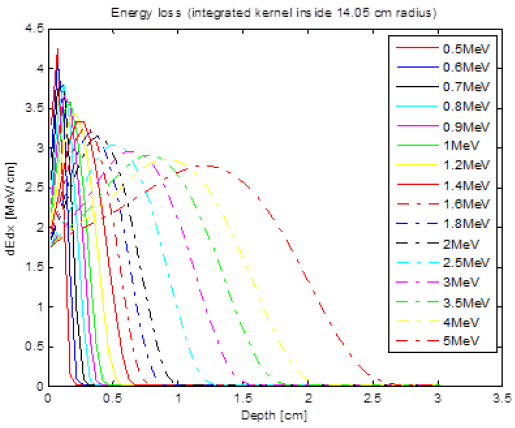
\includegraphics[width=.5\textwidth]{./cap1/electr_enloss.png}
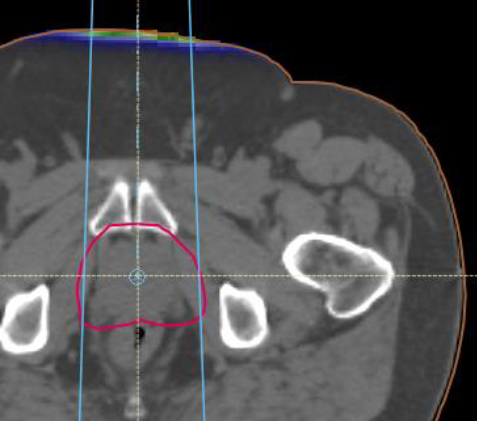
\includegraphics[width=.45\textwidth]{./cap1/electr_doseCT.png}
\caption{Sinistra: diagrammi della dose rilasciata in funzione della profondità di un fascio di elettroni a varie energie. Destra: distribuzione di dose dovuta ad elettroni di contaminazione del fascio calcolata su una CT. Da notare è che questa dose è importante solo nei primi mm di tessuto attraversato.}
\label{fig:electr_enloss}
\end{figure}

L'algoritmo dosimetrico implementato in RayStation per il calcolo della dose da contaminazione elettronica rientra nella classe degli algoritmi \textit{model-based} basati su \textit{convolution/superposition}, con una variante sul kernel di deposizione che non è più puntuale ma esteso di forma cilindrica (vedi Fig.\ref{fig:electr_pencil}). 

\begin{figure}
\centering
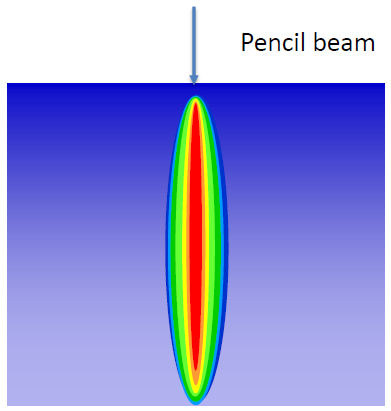
\includegraphics[width=.4\textwidth]{./cap1/electr_pencil.png}$\qquad$
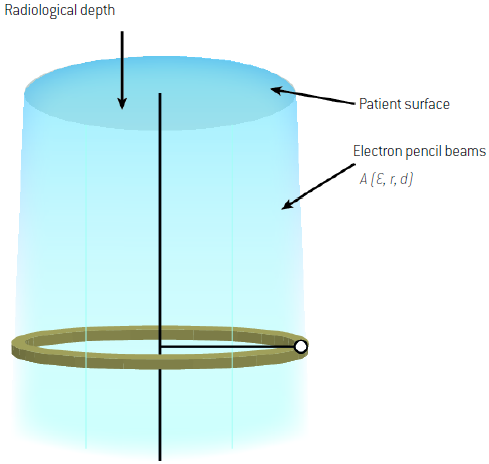
\includegraphics[width=.45\textwidth]{./cap1/electr_pencil_b.png}
\caption{Sinistra: kernel di deposizione di tipo \textit{pencil-beam}. Destra: figura schematica che mostra la simmetria cilindrica nel calcolo della dose quando si utilizza un kernel di tipo \textit{pencil-beam}.}
\label{fig:electr_pencil}
\end{figure}


Questo tipo di algoritmo è denominato \textit{pencil-beam} e rappresenta una versione semplificata del collapsed-cone.\\
L'equazione che permette il calcolo della dose è analoga alla \eqref{eq:superp} rappresentabile semplicemente in coordinate cilindiriche:
\begin{equation}
\label{eq:electr_superp}
D(d) = 2\pi \iint_{E,V} \Psi(r,d,E)\, s(r,d,E)\, r\de r \de E
\end{equation}

L'Eq.\eqref{eq:electr_superp} è implementata all'interno di RayStation in maniera analoga al caso dei fotoni. Schematicamente i passaggi che vengono seguiti sono:
\begin{itemize}
\item I kernel \textit{pencil-beam} sono pre-calcolati con un modello Monte Carlo (software EGSnrc).
\item Viene utilizzato un modello a due sorgenti per calcolare la fluenza di energia elettronica in assenza del paziente.
\item Viene calcolata la distribuzione di TERMA utilizzando la formula della perdita di energia per ionizzazione di Bethe-Bloch per gli elettroni nella materia \cite{RaySearchLaboratories2014}.
\item Vengono applicati i kernel \textit{pencil-beam} per modellizzare lo scatter laterale degli elettroni.
\end{itemize}

Nella Fig.\ref{fig:electr_enloss} è mostrata la distribuzione di dose dovuta agli elettroni di contaminazione calcolata su una CT di un paziente. Questa dose viene sommata alla dose dovuta ai fotoni calcolata con l'algoritmo collapsed-cone. 















